\section{Real-time implementation}
\label{sec:rt}

The application consists of two components:
the first handles importing static GTFS data and constructing the network,
while the second implements the \rt models and prediction.
We used Rcpp \citep{Rcpp}
to develop the program,
which provides access to R \citep{rcore},
which contains many useful tools for data manipulation and package development,
as well as the speed and memory management capabilities of C++.
The program is implemented in the R package
\verb+transitr+, available on Github (\url{https://github.com/tmelliott/transitr}).
In this section, we discuss the features of the \rt component
and assess its performance 
both with respect to timing and travel time estimation.

The general structure of the \rt component is shown below,
with the bold steps being those discussed in this paper.
\begin{enumerate}
\item Load GTFS data from database
\item Each time new data are received \ldots
\begin{enumerate}
    \item Update or create new vehicle objects from the new data
    \item \textbf{Run particle filter on each vehicle to update or initialise its state}
    \item \textbf{Update state of any roads for which vehicles 
        have completed travel}
    \item Generate ETAs for vehicles using combination of vehicle and network state
    \item Write ETAs to a file for distribution
\end{enumerate}
\end{enumerate}


During the development of the application,
we were primarily concerned with ensuring each component of the program
was as efficient as possible,
allowing ETAs to be generated and distributed fast enough to be feasible in real-time,
with a target of 30~seconds or faster at peak time.
Using C++ provided the memory management control necessary to make this possible.
We also made use of OpenMP for parallelisation,
since each vehicle is modelled independently so it is trivial to scale up without
thread safety concerns.


The number of particles needed per vehicle 
depends on many factors,
so it was necessary to explore the performance of the application
with varying number of particles.
Application performance is also assessed
for a range of fixed model parameter values,
such as system noise and GPS error.
To enable comparisons, we implemented a simulated \rt environment
in which the same subset of real vehicle data from 8~October, 2018
could be analysed using a range of settings.
These simulations were carried out of a Virtual Machine 
with 8~cores and 32~Gb of memory, 
running Ubuntu~16.04 and using R~3.4.1.


\subsection{Program Timings}
\label{sec:timings}

In each iteration, 
the timings of the various program components were recorded.
Since the number of vehicles travelling at any given time changes throughout the day,
we used the average timings over an off-peak 15~minute window.
Figure~\ref{fig:timings} shows the average timings for 
varying numbers of particles, $N$.


The most time consuming component was ETA writing,
which involved summarising the individual ETAs estimated for each particle.
While not discussed here this involved computing quantiles which uses a sorting algorithm
with complexity $O(N \log N)$,
which explains non-linear relationship with $N$.


The next most intensive step was vehicle updating,
which took about 5~seconds for 8000 particles.
The ETA prediction step only took a few seconds,
although this may increase once a more comprehensive model is developed.
On our 8-core virtual machine,
the average time to process one iteration during off-peak is about 16~seconds
when 8000~particles are used.
% Figure~\ref{fig:day-timings} shows iteration timings over the course of a day.


\begin{figure}[tb]
    \centering
    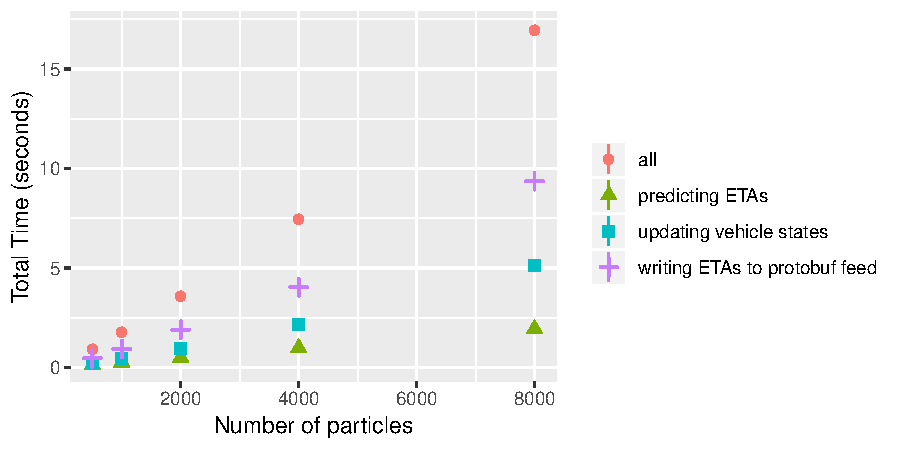
\includegraphics[width=0.8\textwidth]{figures/04_model_results_timing.pdf}
    \caption{
        The average real-time running time of each step within each iteration
        over a 15~minute off-peak window.
        The vehicle update and writing ETA steps involve sorting the particles,
        which is an operation of $\mathcal{O}(N\log N)$ complexity.
        Total time is for the entire iteration, which includes fetching the data from the API.
        % Total time increases as the number of particles $N$ increases.
        % The reason for the large contribution of writing ETAs is that
        % this step involves estimation of quantiles,
        % which requires sorting the particles, 
        % The vehicle update step also involves sorting whenever the sample
        % degenerations and resampling is required.
        % Total time also includes fetching the data from the API,
        % which is constant for any $N$, which explains the increase
        % in standardised total time for $N=500$.
    }
    \label{fig:timings}
\end{figure}




\subsection{Model performance}
\label{sec:model_perf}


To evaluate the performance of the model,
the simulation was run using a range of values of GPS error, $\omega^2$,
and system noise, $\sigma^2$.
Figure \ref{fig:dist_to_route} shows the distribution of the distance
between each observation and the route using a nearest point algorithm,
which suggested using values $\omega \in \{1,2,3,5\}$ for GPS error in meters.
For the system noise we used values of $\sigma^2\in \{1e^{-4},1e^{-3},1e^{-2},0.05\}$,
which correspond to an average vehicle speed variation of between 0.1 and 45~meters per second
over a period of 30~seconds.
For each combination of these parameter values, including varying $N$,
the following values were calculated:
effective sample size, $N_\text{eff}$;
degeneration rate, the percentage of iterations in which the vehicle was lost
(no plausible particles);
and the (relative) variance of segment travel time estimates.


\begin{figure}[tb]
    \centering
    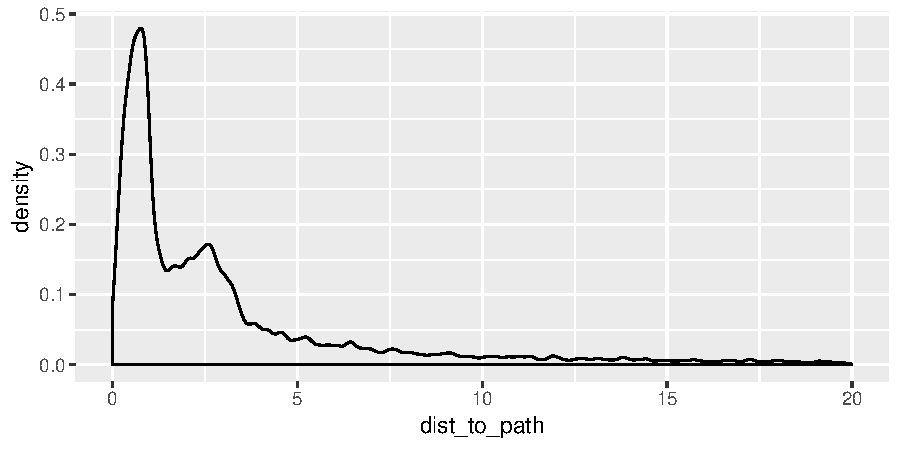
\includegraphics[width=0.8\textwidth]{figures/04_model_results_dist.pdf}
    \caption{
        The distribution of minimum distance between observed vehicle location
        and the route path, truncated to 20~meters.
    }
    \label{fig:dist_to_route}
\end{figure}


Figure~\ref{fig:perf_stats} shows that $N_\text{eff}$ increases
with GPS error and decreases with system noise,
while remaining unaffected by changing $N$.
The degeneration rate decreases with GPS error and increases with $N$,
but is mostly unaffected by system noise.
Large GPS error affects the likelihood,
giving more weight to particles farther from the observation
than does a smaller GPS error.
Conversely, increasing system noise spreads out the particle cloud,
so fewer particles will be near the vehicle,
decreasing $N_\text{eff}$,
but more plausible trajectories are sampled,
so we see a slight decrease in degeneration rate.
Thus, these results are not surprising, 
but show that the model is working as expected.


\begin{figure}[tb]
    \centering
    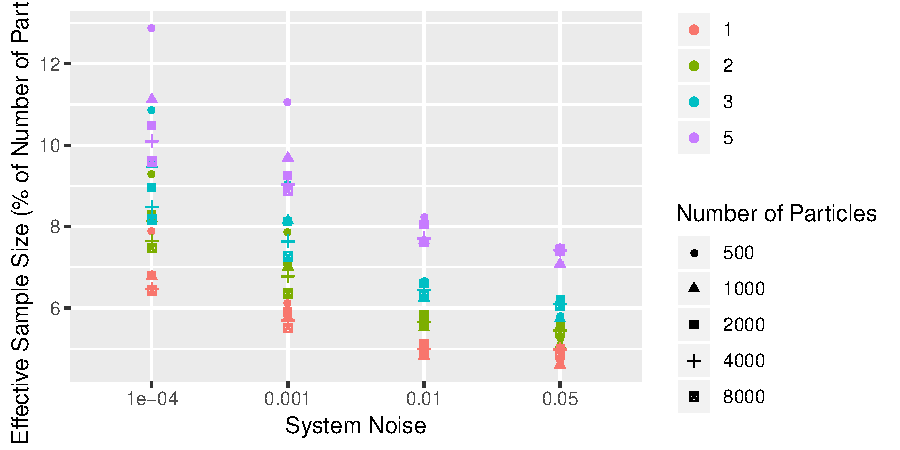
\includegraphics[width=\textwidth]{figures/04_model_results_neff.pdf}
    \caption{
        The effective sample size, $N_\text{eff}$,
        and degeneration rate for varying values of GPS error,
        system noise, and number of particles $N$.
        % increases with GPS error and decreases with system noise,
        % however both effects are reduced for larger $N$.
        % Conversely, degeneration rate decreases with GPS error and
        % system noise, although the effect of the latter is very small,
        % and again the relationship is less pronounced for larger $N$.
    }
    \label{fig:perf_stats}
\end{figure}

% \begin{figure}[tb]
%     \centering
%     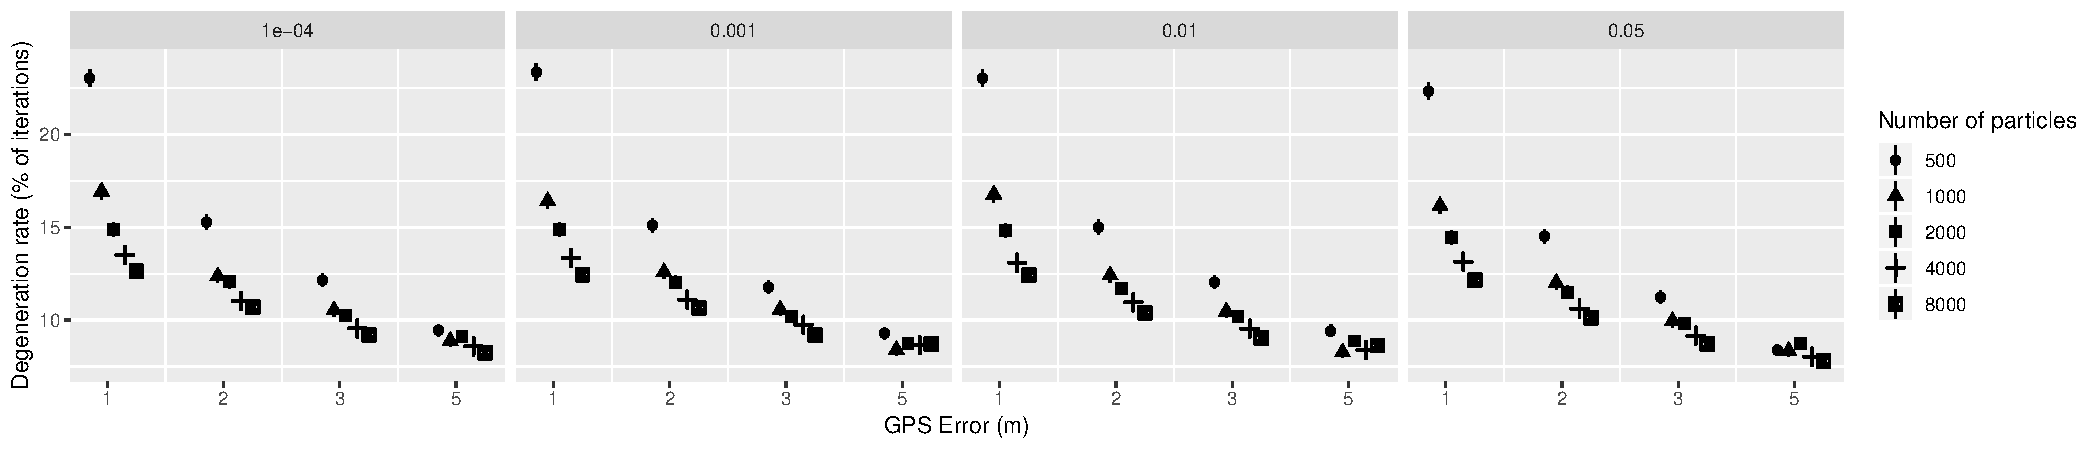
\includegraphics[width=0.9\textwidth]{figures/04_model_results_degen.pdf}
%     \caption{
%         The degeneration rate is the percentage of iterations where there were no
%         plausible particles, so the vehicle was ``lost'' by the model.
%         This decreases as GPS error and number of particles increase,
%         but there is no visible effect of system noise.
%         Note, however, that some of these can be attributed to invalid data,
%         for example if the driver has entered the wrong trip direction.
%         The error bars show $\pm 2$SE.
%     }
%     \label{fig:degen_rate}
% \end{figure}


The last measure of performance is the relative variance of segment travel times.
We used relative variance as each segment has a very different travel time distribution,
so to compare the variability between simulations we needed to 
compute the average variance of estimated travel times over all simulations,
taking the average (over road segments) of the ratio between variance for
each individual simulation and variance over all simulations.
If $\tilde z_\ell^{\omega,\epsilon}$ is a vector of all travel times
along segment $\ell$ during the simulation with GPS error $\omega$ and system noise $\epsilon$,
then the relative variance $\bar v^{\omega,\epsilon}$ is calculated by
\begin{equation*}
\begin{split}
v_\ell^{\omega,\epsilon} &=
\frac{\mathrm{Var}(\tilde z_\ell^{\omega,\epsilon})}{\mathrm{Var}(\tilde z_\ell)} \\
\bar v^{\omega,\epsilon} &=
    \frac{1}{L}\sum_{\ell=1}^L v_\ell^{\omega,\epsilon}
\end{split}
\end{equation*}
Figure~\ref{fig:travel_times} shows that simulations with larger GPS error
resulted in a higher relative variance,
while simulations with more particles had lower relative variance.
There was no visible effect of system noise on the variability of travel times.


The results of the simulations
demonstrate a tradeoff between particle filter performance
($N_\text{eff}$ and degeneration rate) and parameter estimation.
However, until the arrival time prediction model has been completed,
it is difficult to make decisions about the optimal values to use:
we are unable to say whether a higher variation of travel time estimates
is going to have a significant effect on the final ETAs,
particularly when compared to the uncertainty of forecasting road state,
or whether reducing the degeneration rate, 
or increasing $N_\text{eff}$, would be more advantageous.


\begin{figure}[tb]
    \centering
    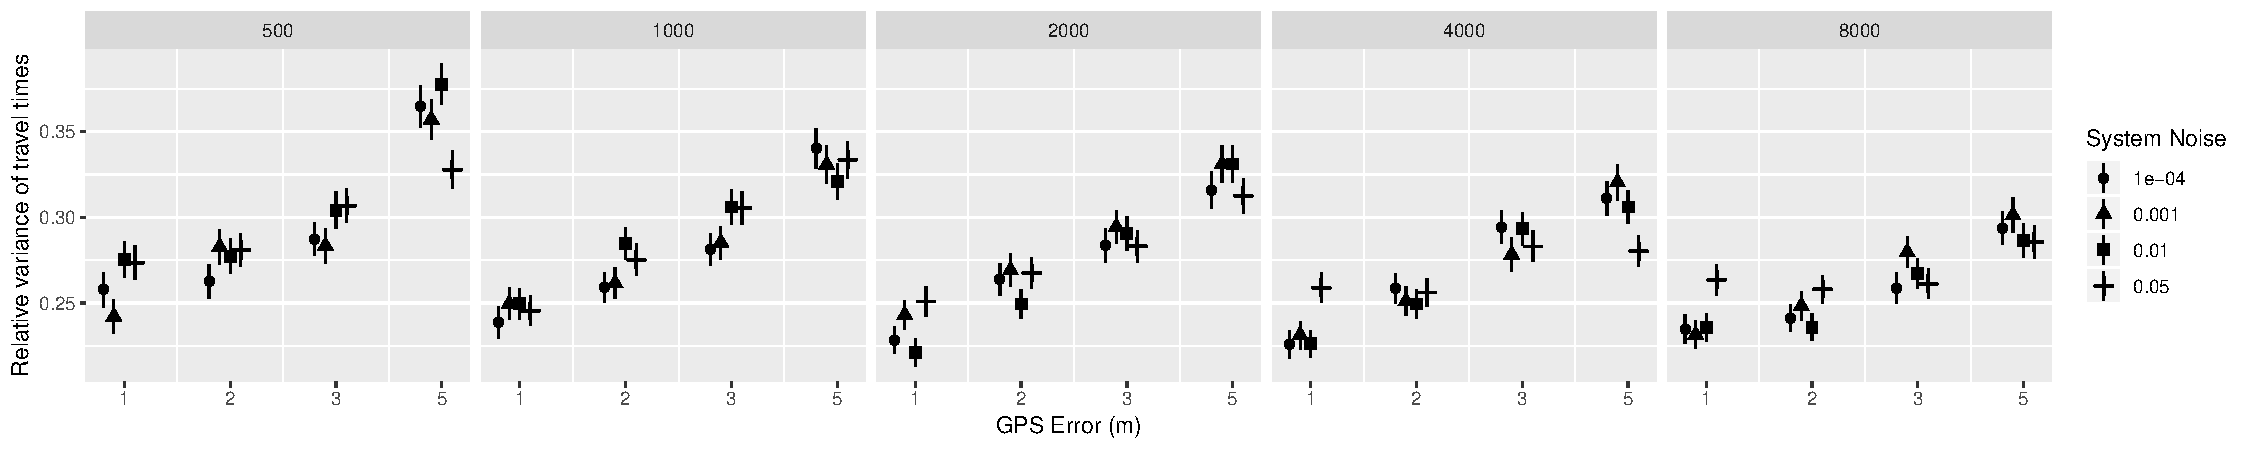
\includegraphics[width=\textwidth]{figures/04_model_results_times.pdf}
    \caption{
        The relative variability of travel time estimates for varying
        values of GPS error, system noise, and number of particles, $N$,
        with error bars $\pm 2$ standard errors.
        % as GPS error increases,
        % with no clear relationship with system noise.
        % Increasing $N$ decreases variability.
    }
    \label{fig:travel_times}
\end{figure}


